\documentclass{beamer}
 
\usepackage[frenchb]{babel}
\usepackage[T1]{fontenc}
\usepackage[utf8]{inputenc}

 
\usetheme{Warsaw}
  
\title{Xmlia : Editeur Xml}
\author []{
\bsc{BOIVIN} Benoit\\
\bsc{LE PHILIPPE} Noé\\
\bsc{KEGBA-SANGO-SANGO} Ulrich-Chancelin\\
\bsc{WOUTERS} Stéphane
}
\institute{}
\date{\today}
\logo{
\includegraphics[height=5mm]{images/logo_um2.png}}

\setbeamertemplate{footline}[frame number]

\AtBeginSection[]
{
  \begin{frame}
  \frametitle{Sommaire}
  \tableofcontents[currentsection, hideothersubsections]
  \end{frame} 
}

\begin{document}

	\begin{frame}
		\titlepage
	\end{frame}

	\section{Présentation du projet}

  \subsection{Editeur XML}

  \begin{frame}
    \frametitle{Editeur XML}
     \begin{itemize}
      \item Le langage XML
      \pause
      \item Le besoin d'un éditeur
      \end{itemize}
  \end{frame}

	\subsection{Cahier des charges}

	\begin{frame}
		\frametitle{Cahier des charges}

    \begin{itemize}
    \item Deux vues
     \begin{itemize}
      \item Vue textuelle
       \pause
         \begin{itemize}
          \item Coloration synthaxique
          \pause
          \item Indentation automatique
          \pause
          \item Auto complétion
          \pause
          \end{itemize}
      \item Vue arborescente
      \pause
          \begin{itemize}
          \item Arbre hiérarchique
           \pause
          \item Actions
           \pause
          \end{itemize}
      \end{itemize}
    \item Validation synthaxique
    \pause
    \item Liason d'un schéma
    \end{itemize}

	\end{frame}

	\subsection{L'existant}

	\begin{frame}
		\frametitle{L'existant}


    \begin{itemize}
    \item De nombreux éditeurs existants
    \pause
       \begin{itemize}
        \item De nombreuses options
        \pause
        \item Payants ou gratuits
        \pause
        \item Un exemple : oXygen
        \end{itemize}
    \end{itemize}


	\end{frame}




	\section{Organisation du projet}

	\subsection{Choix de développement}

	\begin{frame}
		\frametitle{Choix de développement}
	\end{frame}

	\subsection{Fonctionnement du groupe}

	\begin{frame}
		\frametitle{Fonctionnement du groupe}
	\end{frame}




	\section{Développement}
        \subsection{Qt}
	\begin{frame}
	  \frametitle{Présentation de Qt}
          \begin{block}{Qu'est ce que Qt}
            Api orientée objet d'interface graphique
          \end{block}
          \pause
          \begin{block}{Fonctionnement général}
            Un sytème exhaustif de widget
          \end{block}
          \pause
          \begin{block}{De nombreux modules et outils}
            Un grand nombre fonctionnalités déjà présentes
          \end{block}{}
	\end{frame}

        \begin{frame}
          \frametitle{Modèle MVC de Qt}
          \begin{block}{Le modèle}
            Donné par le développeur
          \end{block}
          \pause
          \begin{block}{La vue}
            Gérée par Qt
          \end{block}
          \pause
          \begin{block}{Le contrôleur}
            Un mélange des deux
          \end{block}
        \end{frame}

        \begin{frame}
          \frametitle{Signal/Slot}
          \center
          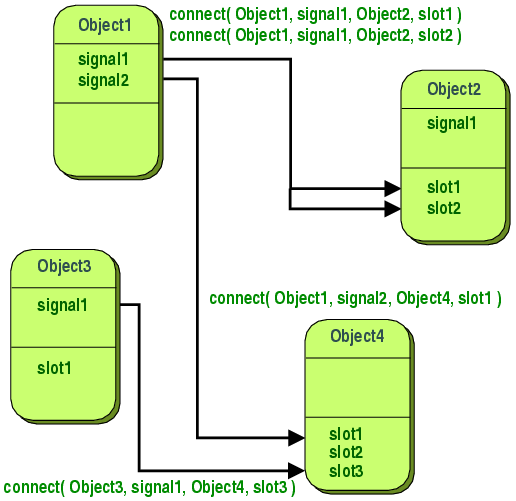
\includegraphics[scale=0.35]{images/abstract-connections.png}
        \end{frame}

        \subsection{Architecture}
        \begin{frame}
          \frametitle{Conception}
          \begin{block}{Choisir nos Widgets}
            Intimement lié à la connaissance de Qt
          \end{block}
          \pause
          \begin{block}{Les faire communiquer}
            Travail asynchrone possible
          \end{block}
        \end{frame}
        
        \begin{frame}
          \frametitle{Communication entre nos composants}
          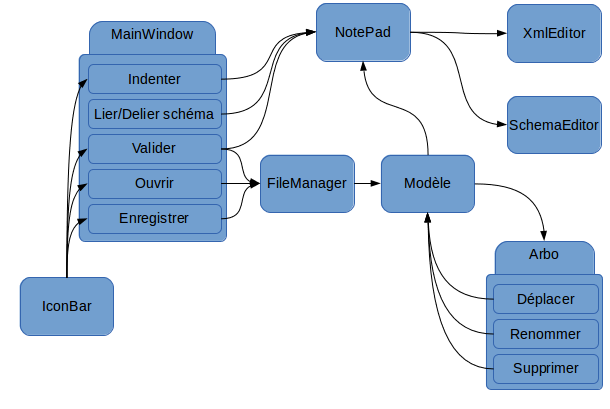
\includegraphics[scale=0.5]{images/communication.png}
        \end{frame}

        \subsection{Les problèmes rencontrés}

        \begin{frame}
          \frametitle{La vue arborescente}
          \begin{block}{L'affichage}
            Modifer le QDomDocument
          \end{block}
          \pause
          \begin{block}{Le glisser-déposer}
            Les signaux de Qt
          \end{block}
        \end{frame}

        \begin{frame}
          \frametitle{L'éditeur de texte}
          \begin{block}{Se repérer dans le texte}
            Correspondance balise/emplacement
          \end{block}
          \pause
          \begin{block}{Manipuler le texte}
            Rester cohérent lors de changements dans l'arborescence
          \end{block}
        \end{frame}
          
	\section{Résultat}

	\begin{frame}
		\frametitle{Résultat}
		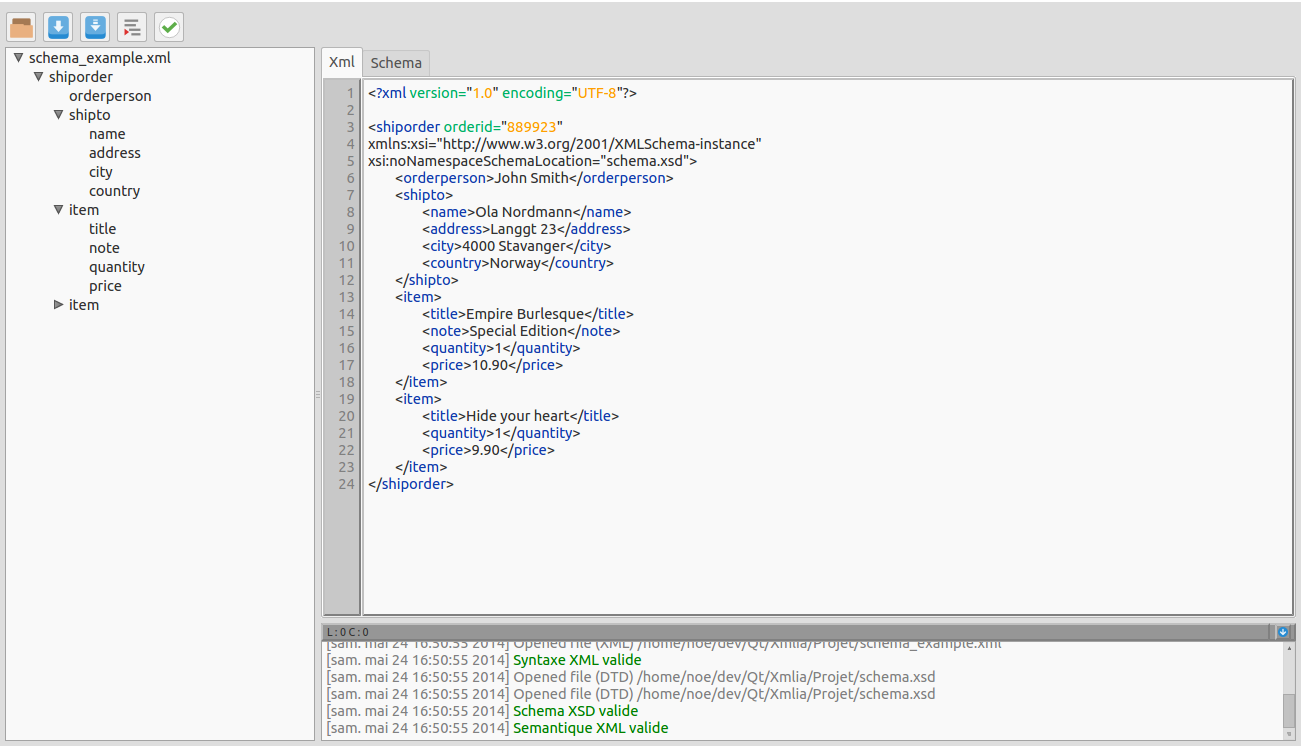
\includegraphics[scale=0.2]{images/final.png}
	\end{frame}


	\section{Conclusion}

	\begin{frame}
		\frametitle{Conclusion}
		\begin{itemize}
			\item Développement sous Qt
			\item Travail en groupe
			\item En bref
		\end{itemize}
	\end{frame}



\end{document}
